\begin{enumerate}[label=\alph*)]
  \item Puisque $A$ est une matrice symétrique, il existe une matrice $V$ orthogonale et une matrice $D$ diagonale dont tous les coefficients sont réels, telles que
  
  \begin{equation*}
    V^{-1} A V = D = \text{diag} \bracket{\lambda_{1}, \dots, \lambda_{n}}
  \end{equation*}
  
  ou, de façon équivalente, $A \BoldV_{i} = \lambda_{i} \BoldV_{i}$ pour $i = 1, \dots, n$, de sorte que les vecteurs colonnes de $V$ soient les vecteurs propres de $A$.
  De plus, les vecteurs propres sont deux à deux orthogonaux (et peuvent être normalisés : donc, on a que $\BoldV_{j}^{\top} \BoldV_{l} = \delta_{jl}$, où $\delta_{jl}$ est le symbole de Kronecker) et on déduit que les vecteurs propres d'une matrice symétrique sont orthogonaux et engendrent l'espace $\R^{n}$ tout entier.


  Donc, soient $\BoldB = \sum_{i = 1}^{n} c_{i} \BoldV_{i}$ le membre de droite du système linéaire $A \BoldX = \BoldB$ et $\BoldX$ sa solution ; en écrivant aussi $\BoldX$ dans la base des vecteurs propres de $A$, on a :
  
  \begin{equation*}
    A \BoldX
    = A \sum_{i = 1}^{n} x_{i} \BoldV_{i} 
    = A \sum_{i = 1}^{n} c_{i} \BoldV_{i}.
  \end{equation*}
  
  Et, puisque $A \BoldV_{i} = \lambda_{i} \BoldV_{i}$, on trouve
  
  \begin{equation*}
    \sum_{i = 1}^{n} x_{i} \lambda_{i} \BoldV_{i} 
    = \sum_{i = 1}^{n} c_{i} \BoldV_{i}.
  \end{equation*}
  
  Donc on trouve
  
  \begin{equation*}
    \sum_{i = 1}^{n} \parent{\lambda_{i} x_{i} - c_{i}} \BoldV_{i} 
    = 0,
  \end{equation*}
  
  c'est-à-dire $\lambda_{i} x_{i} = c_{i}$ et
  
  \begin{equation*}
    \BoldX = \sum_{i = 1}^{n} \parent{c_{i} / \lambda_{i}} \BoldV_{i}.
  \end{equation*}
  
  
  \item Les vecteurs propres de la matrice $A$ sont $\BoldV_{1} = \parent{1, -1}^{\top}$ (qui correspond à $\lambda_{1} = 1$) et $\BoldV_{2} = \parent{1, 1}^{\top}$ (qui correspond à $\lambda_{2} = 2001$).
  Soit $\BoldB = \parent{2001, 2001}^{\top}$ et $\delta \BoldB = \parent{1, 0}^{\top}$.
  Alors,
  
  \begin{equation*}
    \BoldB + \delta + \BoldB
    =   \begin{bmatrix}
          2001 \\
          2001
        \end{bmatrix} 
        +
        \begin{bmatrix}
          1 \\
          0
        \end{bmatrix} 
    = 2001 \BoldV_{2} + \dfrac{1}{2} \parent{\BoldV_{1} + \BoldV_{2}}
    = \dfrac{1}{2} \BoldV_{1} + \dfrac{4003}{2} \BoldV_{2}.
  \end{equation*}
  
  Si on écrit la solution $\BoldX$ comme combinaison linéaire des vecteurs propres, on trouve
  
  \begin{equation*}
    \BoldX
    = \dfrac{\dfrac{1}{2}}{1} \BoldV_{1} + \dfrac{\dfrac{4003}{2}}{2001} \BoldV_{2}
    = \dfrac{1}{2} \BoldV_{1} + \dfrac{4003}{4002} \BoldV_{2}
    \approx 
    \begin{bmatrix}
      1.5 \\
      0.5
    \end{bmatrix}. 
  \end{equation*}
  
  Ainsi on voit que l'erreur $\delta \BoldX$ par rapport à la solution exacte $\BoldX = \parent{1, 1}^{\top}$ est $\delta \BoldX \approx \parent{0.5, -0.5}^{\top}$.
  
  Réciproquement, soit $\BoldB = \parent{1, -1}^{\top}$. La solution exacte du système est $\BoldX = \parent{1, 1}^{\top}$.
  On exprime la solution perturbée par rapport aux vecteurs propres :
  
  \begin{equation*}
    \BoldX + \delta + \BoldX
    =   \begin{bmatrix}
          1.001 \\
          -1
        \end{bmatrix} 
    = \dfrac{2.001}{2} \BoldV_{1} + \dfrac{0.001}{2} \BoldV_{2},
  \end{equation*}
  
  d'où $c_{1} = 2.001/2$ et $c_{2} = 0.001/2$. Donc 
  
  \begin{equation*}
    \BoldB + \delta + \BoldB
    =   \begin{bmatrix}
          2.001 \\
          0
        \end{bmatrix} 
  \end{equation*}
  
  et $\delta \BoldB = \parent{1.001, 1}^{\top}$.
  
  \textit{Remarque.}
  Le système linéaire de cet exercice pourrait être obtenu de l'analyse d'une barre rigide attachée dans sa partie central à un ressort de raideur 4000 et connectée aux extremités à deux ressorts de raideur 1 (voir Figure \ref{fig:ressort} ci-dessous).
  On applique des forces $b_{1}$ et $b_{2}$ aux extremités de la barre et on observe ses déplacements verticaux $x_{1}$ et $x_{2}$.
  Si les forces $b_{1}$ et $b_{2}$ sont équilibrées (par exemple $b_{1} = 2001$, $b_{2} = 2001$), alors de petits changements $\delta \BoldB$ engendrent des mouvements significatifs de la barre (grand $\delta \BoldX$).
  A l'inverse, si les forces ne sont pas équilibrées (par exemple $b_{1} = 1$, $b_{2} = -1$), alors on peut obtenir de petits déplacements $\delta \BoldX$ même si on impose de forts changements $\delta \BoldB$ sur les forces exercées.
  
  \begin{figure}[h!]
    \centering
    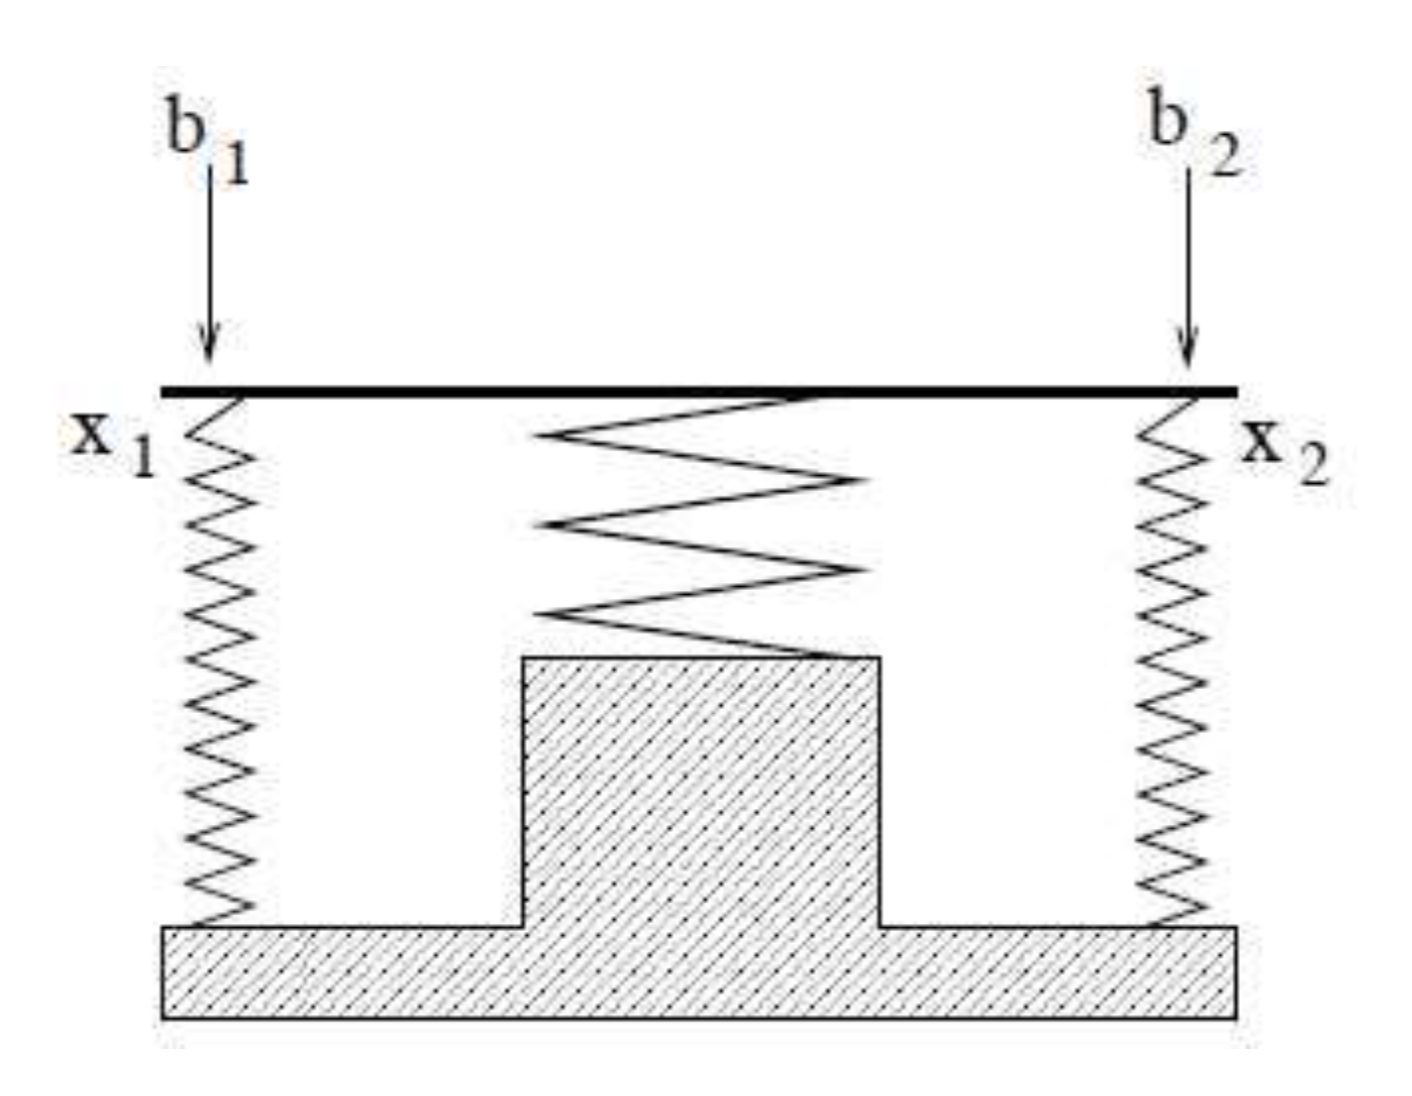
\includegraphics[scale = 0.2]{s2/images/ressort.png}
    \caption{Ressort}
    \label{fig:ressort}
  \end{figure}


\end{enumerate}




